
\section{Objetivos generales}

Para la aplicación de EVS se han marcado las siguientes metas principales:
\begin{itemize}
    \item \textbf{Gestión de la frecuencia de usuarios y eventos en la aplicación.} La aplicación permite gestionar a todos los usuarios en el Sistema
    mediante un usuario Administrador. Esto facilitará la relacion Organización-Cliente mantieniendo un equilibrio entre la cantidad de unos y de otros.
    \item \textbf{Centralizar la planificación de eventos.} La plataforma permite a los usuarios crear y gestionar eventos desde una sola pantalla.
    \item \textbf{Agrupar las Entradas de los usuarios.}  EVS ofrece a los usuarios la posibilidad de Agrupar las entradas en un mismo sitio, así como imprimir las entradas.
    \item \textbf{Aplicación de uso general.} Ofrecer una herramienta para, desde el punto de vista de una organización, mejorar la asistencia a sus eventos
    y, desde el punto de vista del cliente, tener un acceso sencillo e intuitivo a estos.
    \item \textbf{Desarrollo Fullstack.} Aplicar y ampliar los conocimientos adquiridos sobre SpringBoot y Vue.
    \end{itemize}

\section{Descripcón del Problema}
Segun datos oficiales, en España hay 2.922.920 empresas de las cuales solo  5.531 son grandes empresas \cite{pymes} ¿Qué pasa con las 2.917.389 restantes?.

\textbf{Problemas de Comunicación y Alcance:}

\begin{enumerate}
    \item \textbf{Recursos Limitados}: A diferencia de las grandes corporaciones, las PYMEs generalmente no disponen de los mismos recursos financieros 
    y humanos para invertir en estrategias de marketing y comunicación. Esto limita su capacidad para desarrollar campañas efectivas y sostenibles que
    lleguen a una amplia audiencia.
    
    \item \textbf{Falta de Canales de Comunicación Adecuados}: Las grandes empresas suelen tener acceso a una variedad de canales de comunicación, 
    incluidos medios de comunicación masiva, redes sociales gestionadas por equipos especializados y eventos de gran escala. 
    Las PYMEs, por otro lado, a menudo carecen de estos canales, lo que dificulta su capacidad para llegar a nuevos clientes y 
    mantener una comunicación constante con sus públicos objetivo.
    
    \item \textbf{Menor Visibilidad}: Las grandes empresas tienen la ventaja de una mayor visibilidad de marca, 
    lo que les permite mantenerse en la mente de los consumidores más fácilmente. Las PYMEs luchan por obtener y mantener esta visibilidad, 
    lo que puede resultar en una menor lealtad del cliente y dificultades para captar nuevos mercados.
    
    \item \textbf{Tecnología y Digitalización}: Muchas PYMEs no tienen acceso a las últimas tecnologías y herramientas digitales que pueden 
    facilitar la comunicación y el marketing. La falta de digitalización no solo afecta su eficiencia operativa sino también su capacidad para 
    implementar estrategias de marketing digital que son cruciales en el mercado actual.
    
    \item \textbf{Reducción de Costes}: La gestión de eventos corporativos es una herramienta clave para la promoción y la creación de redes, 
    pero muchas PYMEs no pueden permitirse los costes asociados con la organización de eventos a gran escala. Esto limita su capacidad para interactuar cara a cara con clientes potenciales y fortalecer las relaciones comerciales existentes.
    
    \item \textbf{Competencia Intensa}: En un mercado saturado, las PYMEs compiten no solo con otras pequeñas empresas sino también con grandes 
    corporaciones que tienen una presencia más consolidada. La competencia intensa puede hacer que sea aún más difícil para las PYMEs destacar y 
    atraer la atención del público.
\end{enumerate}

\textbf{Impacto en el Crecimiento y Sostenibilidad:}

Estos problemas de comunicación y alcance no solo limitan la capacidad de las PYMEs para crecer, sino que también ponen en riesgo su sostenibilidad 
a largo plazo. Sin los medios adecuados para llegar a su público objetivo y sin una estrategia de comunicación efectiva, estas empresas enfrentan 
dificultades para expandirse, innovar y mantenerse competitivas en el mercado. La falta de visibilidad y la incapacidad para interactuar eficazmente 
con los clientes pueden conducir a una disminución de las ventas y, en última instancia, afectar la viabilidad económica de la empresa.

\textbf{Necesidad de Soluciones Eficientes:}

Para abordar estos desafíos, surge la necesidad de soluciones eficientes y accesibles que puedan ayudar a las PYMEs a mejorar su comunicación y alcance. 
Herramientas que centralicen la gestión de eventos, faciliten la automatización de procesos administrativos, mejoren la visibilidad y proporcionen canales 
de comunicación efectivos son esenciales para permitir que estas empresas compitan en igualdad de condiciones con las grandes corporaciones. 
\textbf{Enterprise Event Solutions} se presenta como una respuesta a estas necesidades, ofreciendo una plataforma integral diseñada específicamente 
para ayudar a las PYMEs a superar sus limitaciones y alcanzar sus objetivos de crecimiento y sostenibilidad.


\section{Estudio de Alternativas}
Contar con las herramientas adecuadas en el campo de la organización de eventos es esencial para el éxito. Debido a su amplia gama de características, 
las aplicaciones de gestión de eventos se han convertido en una herramienta esencial para simplificar tareas, optimizar procesos y 
permitir la realización de eventos memorables.

A continuación se muestra una serie de Aplicaciones Web con funcionalidades parecidas a Enterprise Event Solutions:

\begin{itemize}
    \item \textbf{Eventbrite} es una plataforma versátil para la creación y gestión de eventos. Permite a los usuarios vender entradas online 
    con opciones de precios y tarifas personalizables, así como gestionar el registro y la participación de los asistentes. Además, 
    ofrece herramientas de marketing integradas para promocionar los eventos y análisis de datos detallados sobre la asistencia y 
    el rendimiento de los mismos.
    \item \textbf{Wix Events} es una herramienta de creación de páginas de 
    eventos personalizadas dentro del sitio web de Wix. Ofrece funcionalidades para gestionar el registro de los asistentes y 
    proporciona herramientas de marketing para promocionar los eventos. Además, permite a los usuarios realizar un análisis 
    detallado de la asistencia y el rendimiento del evento a través de datos recopilados en la plataforma.
    \item \textbf{Zoom Events} es una plataforma diseñada para la creación y gestión de eventos virtuales e híbridos, como webinars, 
    reuniones y conferencias. Permite interactuar con los participantes a través de funciones como encuestas, preguntas y respuestas, 
    y chat en vivo. Además, ofrece integraciones con otras herramientas de Zoom para una experiencia más completa y proporciona análisis 
    de datos sobre la asistencia y el rendimiento del evento.
\end{itemize}

El valor añadido distintivo de mi aplicación, \textbf{Enterprise Event Solutions}, reside en el enfoque centrado en el usuario y la excepcional 
facilidad de uso. He diseñado la plataforma desde sus cimientos con la premisa de que la accesibilidad y la usabilidad son fundamentales 
para garantizar una experiencia óptima para todos los usuarios, independientemente de su nivel de familiaridad con la tecnología.

Lo que distingue a \textbf{Enterprise Event Solutions} es la capacidad para llegar a usuarios de todos los niveles de habilidad tecnológica. 
Reconozco que no todos los usuarios están familiarizados con las últimas tecnologías, y es por eso que he priorizado la accesibilidad en el 
diseño de mi plataforma. Incluso aquellos que pueden sentirse desactualizados en términos de tecnología encontrarán que mi aplicación es fácil 
de entender y utilizar, gracias a una interfaz intuitiva que les ayuda a navegar por todas las funcionalidades sin dificultad.

\section{Metodologías Empleadas}

En el desarrollo de Enterprise Event Solutions, he adoptado una metodología ágil basada en Scrum para asegurar que el proceso de creación 
fuera eficiente, organizado y adaptable a cambios y mejoras constantes. Aunque he trabajado solo en este proyecto, he implementado de manera 
rigurosa los principios de Scrum, enfocándome en alcanzar pequeños objetivos semanales y manteniendo una estructura organizada.

Cada semana, he establecido objetivos específicos y alcanzables, lo que me ha permitido avanzar de manera constante y mantener un alto nivel 
de motivación. Esta división en pequeños objetivos semanales me ha ayudado a gestionar mejor el tiempo y a priorizar tareas, asegurando que cada 
funcionalidad de la aplicación se desarrolle de manera coherente y sin omisiones.

Para organizar y seguir mi progreso, he utilizado un tablero de Trello. Este tablero ha sido una herramienta invaluable para no olvidar ideas o 
tareas pendientes. Cada tarjeta en el tablero representaba una tarea o idea específica, y he seguido un flujo de trabajo que incluía las siguientes 
etapas: por hacer, en progreso, y completado. Esta visualización clara del trabajo pendiente y del progreso realizado me ha permitido mantenerme 
enfocado y productivo.

Además, al final de cada semana, he realizado una revisión de los objetivos alcanzados y he ajustado el plan para la semana siguiente. Esta práctica 
de retrospectiva semanal ha sido fundamental para identificar áreas de mejora, solucionar problemas y asegurar que el proyecto siga avanzando de acuerdo 
con los objetivos establecidos.

En resumen, la adopción de la metodología Scrum, con su enfoque en pequeños objetivos semanales y el uso de un tablero Trello para la gestión de 
tareas, ha sido clave para el desarrollo exitoso de Enterprise Event Solutions. A pesar de trabajar solo, esta estructura me ha permitido mantener 
un alto nivel de organización, adaptabilidad y eficiencia en todo el proceso de desarrollo.
\newpage

\begin{figure}[h]
    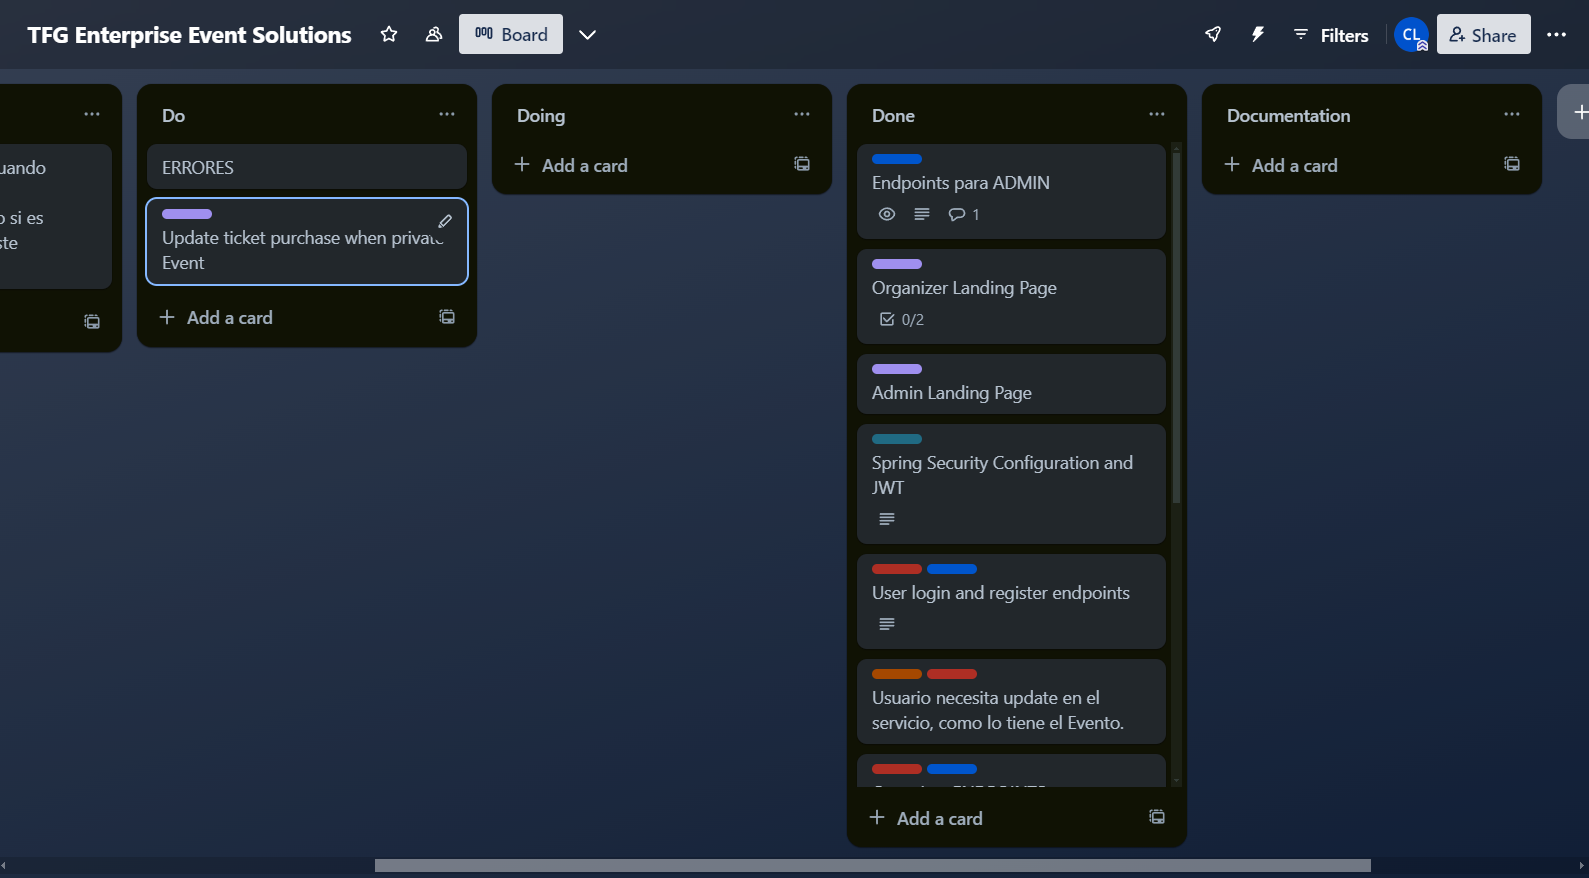
\includegraphics[width=\linewidth]{Trello.png}
    \caption{Trello en proceso.}
    \label{fig:metodologias1}
\end{figure}

En cuanto al desarrollo del código, he utilizado un flujo de trabajo basado en Pull Requests (PRs). Cada cambio o nueva 
funcionalidad se desarrollaba en una rama separada y se integraba al código principal solo después de ser revisada y aprobada 
mediante un Pull Request. Este enfoque me permitió mantener un historial claro de los cambios, realizar revisiones detalladas y 
asegurar que cada nueva adición al código se integrara de manera ordenada y sin conflictos. Aunque he trabajado solo, este método 
me ha ayudado a mantener la disciplina y la organización en el desarrollo del software.

El uso de Pull Requests ha ofrecido múltiples ventajas en el proceso de desarrollo. En primer lugar, ha facilitado la identificación y 
resolución de errores antes de que los cambios se integren en la rama principal. Cada PR actuaba como un punto de control donde podía revisar 
el código, realizar pruebas y verificar la funcionalidad, asegurando que solo los cambios bien testeados y verificados fueran añadidos al proyecto.

Además, este método ha proporcionado una documentación implícita del desarrollo. Cada Pull Request incluía una descripción detallada de los 
cambios realizados, los problemas que solucionaba o las nuevas características añadidas. Esto no solo facilitó la gestión del proyecto, sino 
que también creó un registro histórico útil para futuras referencias y para cualquier otra persona que pueda colaborar en el futuro.

Trabajar con ramas separadas para cada nueva funcionalidad o cambio también ha sido crucial para mantener la estabilidad del proyecto. Al aislar el 
desarrollo de nuevas características en ramas dedicadas, he evitado que los cambios en progreso afecten la estabilidad de la rama principal. Esto ha 
sido especialmente útil para realizar experimentos o implementar grandes cambios sin riesgo de romper la aplicación.

Finalmente, la disciplina de utilizar Pull Requests, incluso trabajando solo, ha fomentado un enfoque metódico y estructurado al desarrollo. Este 
flujo de trabajo me ha obligado a pensar críticamente sobre cada cambio, a documentarlo adecuadamente y a asegurarse de que cada PR cumpliera con los 
estándares de calidad antes de ser fusionado. De hecho, para asegurar que todo cambio que se realizara estuviera controlado por si fuera necesario volver a versiones anteriores
hasta los cambios más pequeños se realizaban mediante PRs. Gracias a esto he consegido revertir cambios en momentos críticos del desarrollo.
\newpage
\begin{figure}[h]
    \centering
    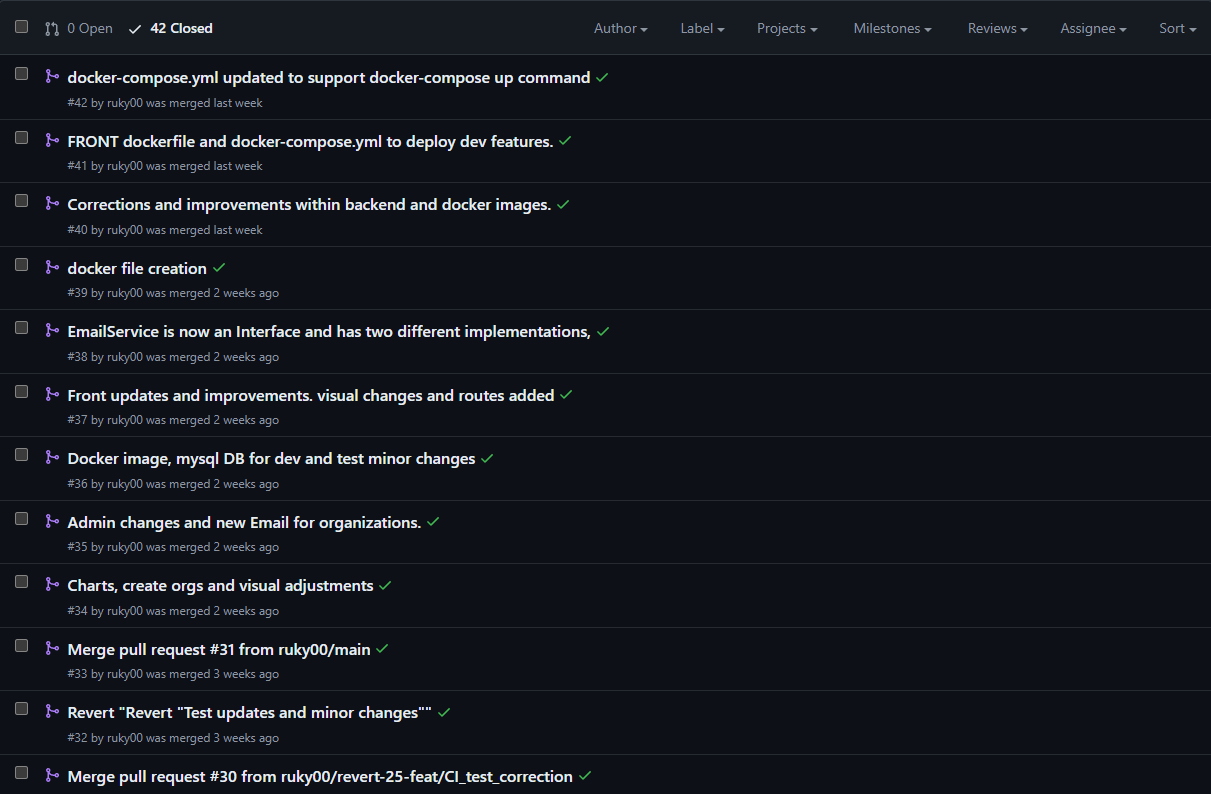
\includegraphics[width=\linewidth]{PRs.png}
    \caption{PRs del Repositorio.}
    \label{fig:metodologias2}
\end{figure}

En resumen, la adopción de la metodología Scrum, con su enfoque en pequeños objetivos semanales y el uso de un tablero Trello para la gestión de tareas, 
junto con el uso de Pull Requests, ha sido clave para el desarrollo exitoso de Enterprise Event Solutions. A pesar de trabajar solo, esta estructura me ha 
permitido mantener un alto nivel de organización, adaptabilidad y eficiencia en todo el proceso de desarrollo. El uso de Pull Requests ha proporcionado un 
marco organizado y eficiente para gestionar y revisar cambios, mantener un historial claro del desarrollo y asegurar la estabilidad y calidad del código.

